\chapter{Considereções Finais}

A evolução do Mezuro não foi motivada por um motivo isolado. Um conjunto de fatores influenciaram e convenceram a equipe que o melhor para o futuro do projeto Mezuro seria um conjunto de modificações em sua estrutura. Os desenvolvedores estavam restritos aos ultrapassados recursos do Rails 2 e do Ruby 1.8, a qual não recebia mais suporte de seus desenvolvedores.

A equipe almejava por liberdade na tomada de decisões, como por exemplo atualizar o Mezuro para as novas versões do Rails e do Ruby, aproveitando suas melhorias e novos recursos. Porém, estavam subordinados as decisões e andamento do projeto Noosfero. A equipe se deu conta que os recursos relacionados a redes sociais fornecidos não eram necessários para uma ferramenta de monitoramento de código-fonte. Além disso, a manutenibilidade e inserção de novos desenvolvedores ao projeto eram tarefas difíceis, já que o Mezuro crescia bastante e se tornava cada vez mais uma aplicação dentro de outra aplicação, ao invés de um plugin com funcionalidades bem específicas.

Levando em conta todos esses fatores, a equipe do Mezuro decidiu retirá-lo do Noosfero, transformando-a em uma aplicação independente, além de formatar uma comunidade de software livre para atrair novos desenvolvedores. Para consolidar esses fatores, que levaram a evolução do Mezuro, foi elaborado um questionário (encontrado no Apêndice \ref{form-pesquisa}) direcionado e equipe que o mantém. Dos fatores que motivaram a evolução, os que mais foram citados pela equipe foram aqueles que limitam sua liberdade ou poder de decisão, que é o fato do Mezuro estar contido dentro do Noosfero, tendo seu desenvolvimento limitado.

A contribuição deste trabalho inclui os seguintes tópicos relacionados a implementação:
\begin{enumerate}
\item ``Manter Repositórios'';
\item ``Manter Configurações'';
\item Melhorias na composição de Configurações, ou seja, o fluxo de adição de métricas de configuração, assim como a edição das mesmas;
\item Adequação da identidade visual, de acordo com as melhores práticas relacionadas à usabilidade;
\item Aplicação de uma técnica de visualização de software;
\end{enumerate}

É importante destacar que, embora o Mezuro esteja evoluindo para uma aplicação distinta do Noosfero, haverá uma integração, ainda a ser discutida pela comunidade de desenvolvedores, entre essas duas ferramentas futuramente.

Os aspectos relevantes deste trabalho não estão restritos apenas aos  pontos práticos ou de implementação citados. A colaboração com um software livre, de acordo com os padrões de contribuição destacados na seção \ref{sec-padroes-sl}, passando por vários dos processos\footnote{Implementação, gerencia de configuração, requisitos e manutenção e evolução de software} que compõem a engenharia de software, além da aplicação de princípios ágeis\footnote{\textit{Pair programming}, divisão de iterações em \textit{sprints}, definição das unidades de trabalho dentro de \textit{backlog}}, interação e envolvimento com uma equipe remota também são pontos notáveis deste trabalho.

%limitações
O código presente no apêndice \ref{radar-chart-code}, referente a técnica de visualização aplicada, o gráfico do radar, se encaixa bem na solução atual que o Mezuro fornece para o processamento de repositórios, que é o processamento de um repositório a cada instante. Porém é desejável que seja apresentado ao usuário o resultado de um ou mais processamentos, para possíveis comparações. Para a visualização dos resultados de mais de um processamento a solução atual não é satisfatória dado que os dados são lidos de um arquivo de extensão \textit{.tsv} onde não é possível separar os dados em grupos que representariam os resultados de cada processamento.

A avaliação de satisfação de usabilidade não pôde ser aplicada aos usuários devido ao fato da plataforma Mezuro estar em um ciclo de desenvolvimento (melhoria) e apesar de estar acessível\footnote{Plataforma Mezuro: http://mezuro.org/}, não é possível completar um ciclo de utilização devido ao módulo de análise do código estar em estado de refatoração em uma mudança de linguagem java para Ruby on Rails.

A quantidade de tecnologias envolvidas para geração de uma nova funcionalidade ou melhoria de um módulo gera uma deadline de aprendizado numa primeira contribuição ao projeto. Porem essa dificuldade é minimizada com a colaboração da equipe para a disseminação de conhecimento.

%continuação
%trabalhos futuros
As funcionalidade e melhorias realizadas no projeto possuem um intuito de continuidade e propagação dos seus benefícios ao longo de outras interfaces pela comunidade da plataforma Mezuro. O padrão gerado na primeira interação foi utilizado por desenvolvedores externos da equipe core a fim de aplicar o comportamento em outras telas que não sofreram a interação conforme citado na subseção \ref{evolucao-usabilidade}. O comportamento dinâmico e com a diminuição de fluxo da funcionalidade Configuration deverá ser aplicado nas funcionalidades New Project, New Configuration e New Repository, por necessitarem de um comportamento similar. Enquanto a visualização, essa deverá ser aplicada para as métricas do projeto ao termino da fase de melhoria de desempenho da análise de código conforme na subseção \ref{visualizacao-software}. Com o termino dessas aplicações, a contribuição dessas melhorias deverá afetar diretamente ou indiretamente aproximadamente 80\% da interface da plataforma.

Pensando em deixar uma perspectiva de trabalhos com foco em usabilidade para uma possível nova interação da comunidade Mezuro uma nova avaliação heurística foi realizada com foco em levantar pontos de melhoria. Os pontos de melhorias levantados foram
\begin{itemize}
\item Feedback ao usuário fixo

Os feedbacks implementados na plataforma conforme Figura \ref{feedback}, modificam a estrutura da tela dificultando ao usuário o que diz respeito a facilidade de memorização, algumas das mensagens necessitam ser encerradas e com o acumulo dessas mensagens o agrupamento e a legibilidade da tela vai se perdendo.

\graphicspath{{figuras/}}
\begin{figure}[h]
\centering
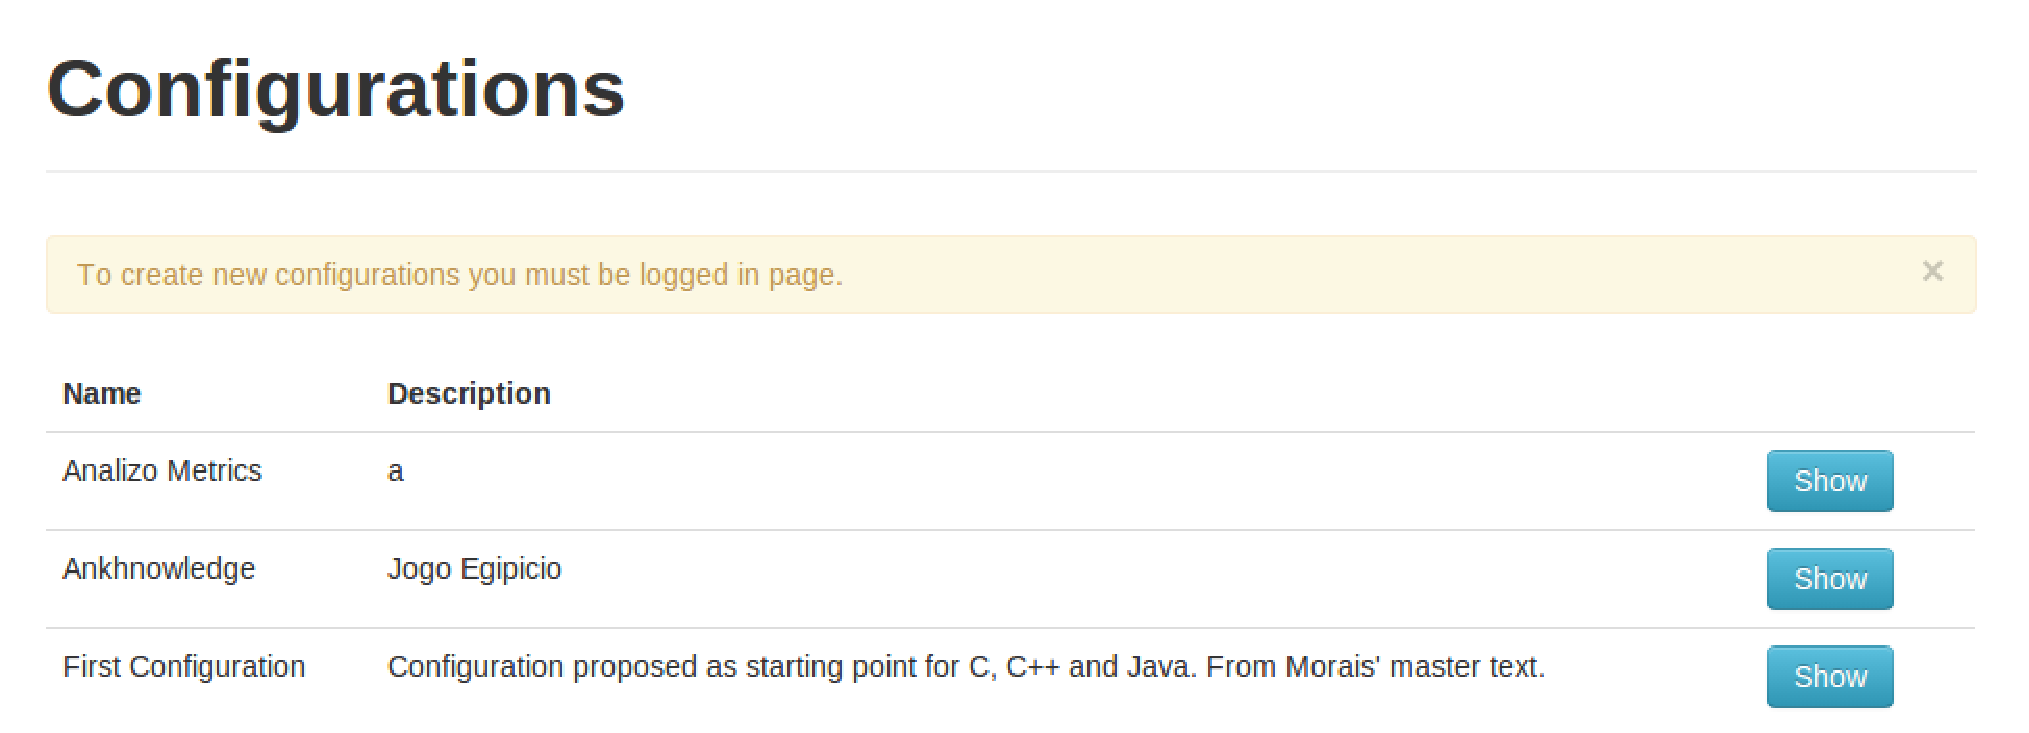
\includegraphics[width=1.0\textwidth]{FeedBack}
\caption{Feedback ao usuário}
\label{feedback}
\end{figure}

O esperado seria mensagens que não alterasse o agrupamento e legibilidade da tela, sem necessitar uma interação do usuário para encerramento dessas mensagens, tendo uma exibição limitada pelo tempo;

\item Feedback com tempo mínimo 

Os feedbacks que não são fixos na tela apresentam tempo inapropriado, pois estão baseados no tempo de processamento das funcionalidades, em um máquina com maior processamentos as mensagens praticamente não são percebidas e a leitura delas não são possíveis. Esse tempo deve ser prefixado para um tempo médio da leitura da mensagem;

\item Internacionalização da plataforma

A plataforma Mezuro é apresentada totalmente na língua inglesa, por ser uma língua amplamente conhecida, porém há uma necessidade de se possibilitar a criação de internacionalização para que a comunidade possa desenvolver dicionários das mensagens em outras línguas e assim aumentar a abrangência do software.

\end{itemize}

%\section{Cronograma}
%
%Para o curto e médio prazo, no escopo deste trabalho, há atividades planejadas para o futuro do Mezuro. Até agora, o Mezuro evoluiu em sua arquitetura, migrando de plugin para aplicação independente com o Rails 4. Na segunda fase deste trabalho, vamos colaborar com novas funcionalidades, que também demandará uma etapa de pesquisa complementar ao que fizemos até agora. As atividades planejadas são:
%
%\begin{enumerate}
%\item Complementação das pesquisas sobre software livre e evolução de software;
%\item Pesquisa sobre visualização de software, formas visuais das métricas de código-fonte;
%\item Colaboração com finalização da migração das funcionalidades do Mezuro Plugin para o novo Mezuro;
%\item Incorporar formas visuais das métricas ao Mezuro (visualizações gráficas);
%\item Implementar suporte a novas linguagens (e.g Ruby);
%\item Escrita do TCC.
%\end{enumerate}
%
%\begin{table}[H]
%\begin{center}
%    \begin{tabular}{ | l | l | l | l | l | l | l | l |}
%    \hline
%    Atividade & Dez 2013 & Jan 2014 & Fev 2014 & Mar 2014 & Abr 2014 & Mai 2014 & Jun 2014 \\ \hline
%    1 & • & • &   &   &   &   &   \\ \hline
%    2 &   & • & • & • &   &   &   \\ \hline
%    3 & • & • & • &   &   &   &   \\ \hline
%    4 &   &   &   & • & • & • &   \\ \hline
%    5 &   &   &   &   &   & • & • \\ \hline
%    6 & • & • & • & • & • & • & • \\ \hline
%    \end{tabular}
%    \caption{Cronograma para atividades do TCC2}
%    \label{tab-cronograma}
%\end{center}
%\end{table}
%
%É importante enfatizar que, após as leituras preliminares e uma avaliação inicial do Mezuro Plugin para a definição do tema e passos para este trabalho, ao final de agosto de 2013, este trabalho começou a ser desenvolvido em setembro de 2013, desde o aprendizado das tecnologias, além dos estudos teóricos para a elaboração deste texto.
%%
%Em 2 meses, conseguimos colaborar efetivamente com o Mezuro ao desenvolver toda a parte de ``gestão de repositório'' de um projeto cadastrado no Mezuro, ou seja, um item central entre as funcionalidades do mesmo.
%%
%Avaliamos que, durante o TCC 1, já percorremos a curva de aprendizado necessária para contribuir com o projeto de Mezuro, para, num primeiro momento, finalizarmos a migração para uma aplicação independente e, posteriormente, inserirmos novas funcionalidades, em especial no contexto de visualização de software, como uma das partes da área de evolução de software que será pesquisada durante o TCC 2 (7 meses, conforme o cronograma apresentado na Tabela \ref{tab-cronograma}).



